\documentclass[11pt,letterpaper]{article}
\usepackage{fontspec}
\usepackage{polyglossia}\setmainlanguage{spanish}
\gappto\captionsspanish{\renewcommand{\figurename}{Figura}\renewcommand{\tablename}{Tabla}\renewcommand{\refname}{Referencias}\renewcommand{\abstractname}{Resumen}}
\setmainfont{TeX Gyre Termes}\setsansfont{TeX Gyre Heros}\setmonofont{TeX Gyre Cursor}
\usepackage[margin=2.4cm]{geometry}
\usepackage{amsmath,amssymb}
\usepackage{graphicx,booktabs,enumitem,xcolor,array}
\usepackage[numbers,sort&compress]{natbib}
\usepackage[font=small,labelfont=bf]{caption}
\usepackage{tikz}\usetikzlibrary{positioning,arrows.meta,fit,calc}
\usepackage{microtype}
\usepackage{lineno}
\usepackage[colorlinks=true,linkcolor=black,citecolor=black,urlcolor=blue!50!black]{hyperref}
\usepackage{authblk}
\renewcommand\Affilfont{\small}\renewcommand\Authand{ y }\renewcommand\Authands{ y }
\setlength{\parskip}{2pt}
\linenumbers

\title{\bfseries Alta exactitud interna, desempeño externo al nivel del azar: validación externa preregistrada de la selección de electrodos con NSGA-II para detectar deterioro cognitivo leve con EEG}
\author[1]{Jessica Milagros Cordero Rivera}
\author[1,*]{Ana Carolina Torres Villegas}
\author[1]{Salvador Miguel Hinojosa Cervantes}
\affil[1]{Tecnológico de Monterrey, Campus Guadalajara, Zapopan, Jalisco, Mexico}
\affil[*]{Autora de correspondencia: \href{mailto:torresvillegasanacarolina@gmail.com}{torresvillegasanacarolina@gmail.com}}
\date{}

\begin{document}
\maketitle

\begin{abstract}
\noindent\textbf{Antecedentes.} Un estudio reciente reportó hasta 95\,\% de exactitud para detectar deterioro cognitivo leve (MCI) con EEG en reposo usando 5--7 electrodos elegidos por un algoritmo genético multiobjetivo (NSGA-II), con validación \emph{leave-one-subject-out} en 24 personas. La selección y la evaluación usaron a las mismas personas y no hubo prueba externa.
\textbf{Métodos.} Reconstruimos el método de forma independiente y usamos la base pública original (EEG\_1) solo para desarrollo, donde cuantificamos la fuga entre segmentos, el sesgo de selección y la contaminación ocular. Congelamos la réplica y cuatro alternativas (potencia relativa por banda limpia con ICA y LDA con contracción: sin selección, con un electrodo por zona, con NSGA-II y con un enjambre de partículas binario penalizado), preregistramos en OSF hipótesis, reglas de decisión y huellas del código, y probamos cada método una sola vez en una base pública independiente del mismo centro y equipo (EEG\_2; 18 MCI, 16 controles). Un análisis secundario usó un montaje físico procesado canal por canal.
\textbf{Resultados.} En desarrollo, mezclar segmentos de la misma persona elevó la exactitud de 50--57\,\% a 90--99\,\%, y NSGA-II alcanzó 72--79\,\% con etiquetas revueltas. En la prueba externa, la exactitud interna de 75.1\,\% de la réplica cayó a una exactitud balanceada de 45.8\,\% (IC 95\,\% 31.2--60.1), lo que confirmó la primera hipótesis. Ningún método superó el azar ($p_\text{Holm}=1.00$); las cuatro alternativas predijeron MCI para las 34 personas, por lo que su no inferioridad formal fue trivial. Las dos bases se distinguieron en 94.4\,\% solo con las características del EEG: EEG\_2 estaba dominada por actividad delta (69\,\% frente a 40\,\% de la potencia de 1--30\,Hz) y la interferencia de la red eléctrica se asoció con el diagnóstico en sentidos opuestos en cada base. Los AUC externos fueron de 0.40--0.52 y la estandarización por base no reveló señal residual. La comparación con el montaje físico fue no concluyente.
\textbf{Conclusiones.} Las exactitudes reportadas no se transfirieron a personas nuevas. El cambio de dominio y los confusores de adquisición pesaron más que cualquier señal relacionada con el MCI. La minimización de electrodos debe venir después, no antes, de una validación por persona, anidada y externa preregistrada.\\[4pt]
\noindent\textbf{Palabras clave:} deterioro cognitivo leve; EEG; selección de canales; NSGA-II; validación externa; preregistro; réplica; cambio de dominio.
\end{abstract}

\begin{figure}[t]
\centering\resizebox{\linewidth}{!}{%
\begin{tikzpicture}[every node/.style={font=\scriptsize, align=center},
  box/.style={draw, rounded corners=2pt, minimum height=13mm, text width=27mm, fill=#1}, box/.default=gray!8,
  arr/.style={-{Stealth[length=2mm]}, thick}]
\node[box=blue!8]   (d1)  at (0,0)     {\textbf{EEG\_1}\\24 personas\\(11 MCI, 13 controles)};
\node[box]          (dev) at (3.6,0)   {\textbf{Desarrollo}\\réplica\\+ controles diagnósticos};
\node[box]          (frz) at (7.2,0)   {\textbf{Congelar}\\R, M0, M4, M1, M6\\+ montaje físico};
\node[box=orange!12](reg) at (10.8,0)  {\textbf{Preregistro}\\hipótesis, reglas,\\SHA-256 de código y datos};
\node[box=blue!8]   (d2)  at (14.4,0)  {\textbf{EEG\_2}\\34 personas\\(18 MCI, 16 controles)};
\node[box=orange!12, text width=52mm] (tst) at (12.6,-2.4) {\textbf{Prueba externa única}\\ajuste con EEG\_1, predicción de EEG\_2 una vez;\\un script aplica las reglas registradas};
\draw[arr] (d1) -- (dev); \draw[arr] (dev) -- (frz); \draw[arr] (frz) -- (reg);
\draw[arr] (reg.south) -- (reg.south |- tst.north); \draw[arr] (d2.south) -- (d2.south |- tst.north);
\draw[dashed, gray] (12.6,1.0) -- (12.6,-0.9); \node[font=\tiny, text=gray] at (12.6,1.25) {sin acceso antes del registro};
\end{tikzpicture}}
\caption{\textbf{Diseño del estudio.} EEG\_1 se usó para todo lo que implica decisiones; EEG\_2 se usó una sola vez, después del preregistro, con código congelado.}
\label{fig:design}
\end{figure}

\section{Introducción}

El deterioro cognitivo leve (MCI, por sus siglas en inglés) es una disminución de la cognición mayor a la esperada para la edad que todavía no compromete la independencia, y con frecuencia precede a la demencia \citep{petersen2004}. El electroencefalograma (EEG) en reposo es atractivo para el tamizaje porque es barato, no invasivo y portátil, y porque el MCI y la enfermedad de Alzheimer se asocian con un enlentecimiento de los ritmos de reposo, en particular con menor potencia alfa posterior \citep{babiloni2015,cassani2018}. Un dispositivo de tamizaje sería más práctico con pocos electrodos, por lo que varios estudios buscan el montaje más pequeño que conserve la exactitud diagnóstica.

\citet{aljalal2024} abordaron esta pregunta con un algoritmo genético multiobjetivo (NSGA-II; \citealp{deb2002}) que busca los electrodos y las características que maximizan la exactitud con validación \emph{leave-one-subject-out} (LOSO) mientras minimizan el número de electrodos. Con una base pública de 24 personas de Isfahan \citep{kashefpoor2016} reportaron 89.7\,\% de exactitud con los 19 electrodos, hasta 94.9\,\% con 7 electrodos y hasta 95.8\,\% al seleccionar también características. Los electrodos elegidos con más frecuencia fueron Cz, F8, T4 y Fp1. El código no se publicó.

Tres problemas bien documentados pueden inflar estas cifras. Primero, cuando segmentos de una misma persona quedan a la vez en entrenamiento y prueba, el clasificador puede reconocer a la persona en lugar de la condición \citep{saeb2017}. Segundo, cuando la misma estimación de validación cruzada se usa para elegir un modelo (aquí, el subconjunto de electrodos) y para reportar su desempeño, el valor reportado tiene un sesgo optimista que crece con el número de modelos candidatos \citep{varma2006,cawley2010}. NSGA-II evalúa miles de subconjuntos, así que este sesgo de selección puede ser grande. Tercero, con unas pocas decenas de personas el error de muestreo de cualquier exactitud es amplio, de alrededor de $\pm 15$ puntos porcentuales \citep{varoquaux2018}, de modo que el azar produce mejoras aparentes con facilidad. Un cuarto problema, propio del área, concierne a los electrodos frontales: Fp1, Fp2, F7 y F8 registran movimientos oculares, que pueden diferir entre grupos y actuar como variable de confusión. Por último, los electrodos elegidos después de una referencia promedio y un análisis de componentes independientes (ICA) calculados con los 19 canales son \emph{virtuales}: su señal contiene información de los demás electrodos y un dispositivo con solo esos electrodos no podría reproducirla.

La única forma de saber si un montaje seleccionado generaliza es probarlo una vez en personas que nunca se usaron para construirlo ni elegirlo \citep{collins2024}. Por eso (i) reconstruimos de forma independiente en Python el método de \citet{aljalal2024}; (ii) usamos la base original (EEG\_1) solo para desarrollo, donde cuantificamos los problemas anteriores con controles diagnósticos; (iii) congelamos la réplica y cuatro alternativas diseñadas para atenderlos; (iv) preregistramos hipótesis, reglas de decisión y huellas del código \citep{nosek2018,osfprereg}; y (v) hicimos una única prueba externa en una base pública independiente del mismo centro y equipo (EEG\_2; \citealp{kashefpoor2019}). Un análisis secundario, también preregistrado, evaluó si las conclusiones se sostienen con un montaje físico, en el que cada electrodo se procesa por separado.

\section{Materiales y métodos}

\subsection{Bases de datos}

Ambas bases son registros públicos de EEG en reposo de la Universidad de Ciencias Médicas de Isfahan, adquiridos con el mismo sistema (19 electrodos del sistema 10--20, 256\,Hz, unos 30 minutos por registro) y distribuidos por el mismo grupo \citep{kashefpoor2016,kashefpoor2019}. La Tabla~\ref{tab:data} las resume. Según la fuente, el MCI se diagnosticó con una entrevista neuropsiquiátrica basada en los criterios de Petersen, con puntajes del Mini-Mental State Examination (MMSE) de 21 a 26 para MCI y mayores de 26 para controles; los participantes tenían de 60 a 77 años y se habían sometido a una angiografía coronaria en el año previo. EEG\_2 se publicó como extensión de la misma base; no pudimos verificar que sus criterios de inclusión sean idénticos. Los estudios originales obtuvieron aprobación ética y consentimiento informado según se reporta en sus publicaciones; el presente trabajo es un análisis secundario de datos públicos anonimizados.

\begin{table}[t]
\centering\small
\caption{\textbf{Bases de datos.} Ambas provienen del mismo centro y sistema de registro. Las etiquetas se leyeron del archivo \texttt{states.xlsx} de cada base.}
\label{tab:data}
\begin{tabular}{@{}lll@{}}
\toprule
 & EEG\_1 (desarrollo) & EEG\_2 (prueba externa) \\
\midrule
Personas disponibles & 27 (11 MCI, 16 controles) & 34 (18 MCI, 16 controles) \\
Personas usadas & 24 (11 MCI, 13 controles)\textsuperscript{a} & 34 (sin exclusiones) \\
Duración del registro & unos 30 min & 27.3--37.9 min \\
Segmentos por persona & 60 $\times$ 10\,s (primeros 10 min) & 60 $\times$ 10\,s (primeros 10 min) \\
Función & solo desarrollo y selección & prueba única y bloqueada \\
Referencia & \citet{kashefpoor2016} & \citet{kashefpoor2019} \\
\bottomrule
\end{tabular}

\smallskip\footnotesize\raggedright \textsuperscript{a}\,\citet{aljalal2024} excluyeron a tres controles sin identificarlos; nosotros excluimos a los tres controles con más segmentos de 10\,s por encima de 100\,\textmu V (HC\_12, HC\_17, HC\_24). El análisis con las 27 personas se reporta como exploratorio.
\end{table}

Antes de la prueba externa verificamos que ningún registro de EEG\_2 duplicara uno de EEG\_1: ningún archivo es idéntico (MD5) y la correlación máxima entre cualquier fragmento de 30\,s de EEG\_2 y cualquier registro de EEG\_1 fue de 0.74, frente a 1.00 de una copia. Los 34 registros de EEG\_2 tienen los 19 canales a 256\,Hz y duran más de 10 minutos.

\subsection{Réplica independiente del método original}

Reconstruimos el procedimiento de \citet{aljalal2024} a partir de su sección de métodos (Fig.~\ref{fig:design}). Los primeros 10 minutos de cada registro se filtraron con un pasa-banda de 0.5--64\,Hz, se re-referenciaron al promedio común, se les aplicó un filtro notch en 50 y 100\,Hz y se dividieron en 60 segmentos de 10\,s. Cada segmento se descompuso con una transformada wavelet discreta de cinco niveles (Daubechies-4, sin el detalle D1; \citealp{mallat1989}) o con descomposición variacional de modos, y en cada sub-banda y canal se calcularon diez medidas (entre ellas la entropía de umbral, ThEn, y la energía de Teager, TeEng). Cuatro clasificadores (\emph{k} vecinos más cercanos, máquina de vectores de soporte, análisis discriminante y bosque aleatorio) se evaluaron con LOSO, promediando la exactitud de los segmentos de cada persona como en el artículo original. NSGA-II usó un cromosoma binario sobre los 19 canales más genes enteros para los hiperparámetros del clasificador, con los dos objetivos del artículo: menos canales y mayor exactitud LOSO. Para la selección de canales, la población y las generaciones fueron 200 y 50. Las decisiones que el artículo original no especifica (familia wavelet, umbral de ThEn de 2\,\textmu V, operadores genéticos, estandarización dentro de cada pliegue, qué controles excluir) están documentadas en el código. La réplica corrida en dos computadoras distintas dio resultados idénticos en las 80 combinaciones de medida, descomposición y clasificador.

\subsection{Controles diagnósticos en los datos de desarrollo}

Solo con EEG\_1 cuantificamos los problemas descritos en la Introducción: (i) validación cruzada de 10 particiones por registro, que mezcla segmentos de la misma persona, frente a LOSO por persona; (ii) NSGA-II con etiquetas diagnósticas revueltas, que muestra la exactitud que alcanza la búsqueda sin ninguna señal real \citep{ojala2010}; (iii) LOSO anidado, en el que NSGA-II elige electrodos con 23 personas y el modelo elegido se prueba en la 24.ª, 24 veces \citep{varma2006}; y (iv) el contenido ocular de cada electrodo, estimado como la fracción de su varianza explicada por los componentes de ICA más correlacionados con electrooculogramas vertical y horizontal derivados de los canales frontales \citep{jung2000}.

\subsection{Métodos comparados en la prueba externa}

Cinco métodos quedaron congelados en el código antes del preregistro (Tabla~\ref{tab:methods}). R es la réplica de \citet{aljalal2024} en su mejor configuración reportada para selección de canales (DWT, ThEn, análisis discriminante), con la regla del artículo de quedarse con la solución de mayor exactitud interna. M0, M4, M1 y M6 comparten una representación más limpia diseñada para atender los problemas: (a) eliminación por ICA de los dos componentes más correlacionados con los movimientos oculares vertical y horizontal, exclusión de Fp1, Fp2, F7 y F8 y recálculo de la referencia promedio; (b) características que la literatura asocia con el MCI, el logaritmo de la potencia relativa en las bandas delta (1--4\,Hz), theta (4--8\,Hz), alfa (8--13\,Hz) y beta (13--30\,Hz), calculada con el método de Welch \citep{welch1967} en cada segmento de 10\,s y promediada por persona, para que la unidad de análisis sea la persona y no el segmento; y (c) un clasificador regularizado, el análisis discriminante lineal (LDA) con contracción de Ledoit--Wolf \citep{ledoit2004}. M0 usa los 15 electrodos restantes sin selección. M4 restringe la búsqueda a un electrodo por zona del cuero cabelludo (frontal, central, temporal y parieto-occipital; 180 combinaciones evaluadas exhaustivamente), un espacio de búsqueda mucho menor que deja menos oportunidades de ajustar ruido. M1 aplica NSGA-II con la regla del artículo a las mismas características. M6 usa optimización por enjambre de partículas binaria \citep{kennedy1997} con una penalización explícita de un punto porcentual por electrodo, para comprobar que las conclusiones no dependen del algoritmo de búsqueda \citep{wolpert1997}. En M1 y M6 la predicción de cada persona es el voto de mayoría de cinco semillas. Toda la selección dentro de M4, M1 y M6 usa un \emph{leave-one-out} interno sobre las personas de entrenamiento.

\begin{table}[t]
\centering\footnotesize
\caption{\textbf{Métodos congelados antes de la prueba externa.} Todos se ajustan y eligen sus electrodos solo con EEG\_1. LDA: análisis discriminante lineal; LOO: \emph{leave-one-out}.}
\label{tab:methods}
\begin{tabular}{@{}p{1.7cm}p{3.6cm}p{3.1cm}p{5.4cm}@{}}
\toprule
Método & Señal & Características & Selección de electrodos y decisión \\
\midrule
R & 19 canales, referencia promedio & ThEn de DWT por segmento & NSGA-II (200$\times$50, semilla 0), mayor exactitud LOSO interna; etiqueta de la persona = mayoría de sus segmentos \\
M0 & Limpia con ICA, 15 canales\textsuperscript{a} & Log de potencia relativa por banda, promedio por persona & Ninguna (15 electrodos); LDA con contracción \\
M4 & Como M0 & Como M0 & Un electrodo por zona, búsqueda exhaustiva (180), exactitud balanceada LOO interna \\
M1 & Como M0 & Como M0 & NSGA-II (40$\times$25) con la regla del artículo; voto de 5 semillas \\
M6 & Como M0 & Como M0 & PSO binario (20 partículas, 25 iteraciones), aptitud = exactitud balanceada interna $-$ 1 punto por electrodo; voto de 5 semillas \\
M0 y M4 físicos & 15 canales, solo filtrado por canal (sin referencia promedio ni ICA) & Como M0 & Como M0 y M4 \\
\bottomrule
\end{tabular}

\smallskip\raggedright \textsuperscript{a}\,Fp1, Fp2, F7 y F8 se eliminan después de la ICA; se recalcula la referencia promedio.
\end{table}

\paragraph{Montaje físico.} En M0 y M4 las características de cada electrodo se calculan después de una referencia promedio y una ICA estimadas con los 19 canales. Para probar si el ahorro de electrodos se sostiene con electrodos reales, M0-físico y M4-físico repiten M0 y M4 solo con operaciones de un canal (filtros pasa-banda y notch), conservando la referencia original del registro. Este análisis se agregó después de congelar los métodos principales y se preregistró como secundario.

\subsection{Preregistro y prueba externa}

Las hipótesis, las reglas de decisión, el código (huella SHA-256 de cada archivo) y los archivos de características extraídas de EEG\_2 (también fijados por SHA-256; la extracción es determinista y los reproduce bit a bit) se registraron en OSF antes de entrenar o evaluar cualquier modelo con EEG\_2 \citep{osfprereg}. Después se corrió la prueba externa una sola vez: cada método se ajustó con EEG\_1 y predijo a cada persona de EEG\_2, y un script aplicó las reglas de decisión preregistradas a las predicciones guardadas.

La medida principal fue la exactitud balanceada por persona en las 34 personas de EEG\_2, es decir, el promedio de sensibilidad y especificidad. La pregunta de investigación (PI) fue qué métodos superan el azar; se fijaron las predicciones de cada método y se permutaron las etiquetas de prueba 10\,000 veces, con corrección de Holm sobre los cinco métodos \citep{holm1979}. Se registraron cuatro hipótesis:
\begin{itemize}[leftmargin=*,itemsep=1pt]
\item \textbf{H1.} R muestra alta exactitud interna pero mucho menor exactitud externa. Se confirma si la exactitud LOSO interna de R (la cifra que reportaría el artículo original) queda por encima del límite superior del intervalo de confianza (IC) bootstrap del 95\,\% de su exactitud balanceada externa.
\item \textbf{H2.} M0 no es inferior a R.
\item \textbf{H3.} M4 y M6 no son inferiores a M1 y usan menos electrodos (mediana entre semillas).
\item \textbf{H4 (secundaria).} M0-físico no es inferior a M0 con ICA. Como M4-físico cayó a 36.7\,\% en desarrollo (Sección~\ref{sec:dev}), no se hizo predicción para él.
\end{itemize}
La no inferioridad \citep{walker2011} usó un margen de $-10$ puntos porcentuales de exactitud balanceada, la menor pérdida que consideramos relevante para un tamizaje y aproximadamente la ganancia que dio la limpieza de artefactos en desarrollo. Se evaluó con un bootstrap pareado de personas estratificado por clase (10\,000 remuestreos; \citealp{efron1993}); se concluyó no inferioridad si menos del 5\,\% de las diferencias remuestreadas quedaban en $-10$ o por debajo, es decir, si el límite inferior del IC bilateral del 90\,\% quedaba por encima de $-10$. Se aplicó corrección de Holm a las dos comparaciones de H3 y, por separado, a las de H4. Para la exactitud simple se reportan intervalos exactos de Clopper--Pearson \citep{clopper1934}. Con 18 MCI y 16 controles, un método necesita al menos 62\,\% de exactitud balanceada para superar el azar; la potencia para detectar exactitudes balanceadas reales de 60, 70 y 80\,\% es 0.40, 0.84 y 0.99 (simulación). Un IC que contiene a la vez $-10$ y 0 se reporta como no concluyente.

Como control descriptivo del cambio de dominio, un LDA con contracción y \emph{leave-one-out} intentó distinguir, solo con las características de 15 electrodos, de qué base provenía cada una de las 58 personas (\emph{efecto de base}).

\subsection{Análisis exploratorios}

Los siguientes análisis se declararon exploratorios en el preregistro: (i) la prueba externa de M0 y M4 entrenados con las 27 personas de EEG\_1; (ii) el área bajo la curva ROC (AUC), estimada con \emph{leave-pair-out} en EEG\_1 \citep{airola2011} y externamente en los métodos con puntaje continuo; (iii) la interferencia de la red eléctrica, medida como el logaritmo del cociente entre la potencia en 49--51\,Hz y la potencia en 1--45\,Hz de los registros originales, y la actividad lenta frontal (potencia en 0.5--4\,Hz en Fp1, Fp2, F7 y F8), ambas comparadas entre grupos y entre bases; (iv) un control positivo: la dirección de la diferencia entre grupos en la potencia alfa relativa posterior (P3, Pz, P4, O1, O2), que se espera menor en MCI \citep{babiloni2015}; y (v) la estabilidad de los electrodos elegidos por M1 y M6 entre semillas.

\subsection{Software y reproducibilidad}

Todos los análisis se corrieron en Python con MNE-Python \citep{gramfort2013}, scikit-learn \citep{pedregosa2011}, NumPy y SciPy. NSGA-II y el PSO binario se implementaron a partir de sus descripciones originales. Todos los pasos aleatorios usan semillas fijas. El código, el preregistro y los resultados están disponibles en el registro de OSF y en el repositorio que acompaña al artículo.

\section{Resultados}

\subsection{Datos de desarrollo (EEG\_1)}\label{sec:dev}

\paragraph{Mezclar segmentos de la misma persona explica la mayor parte de la exactitud reportada.} Con los 19 canales y LOSO por persona, la réplica obtuvo 49.9--56.6\,\% (exactitud de segmentos promediada por persona) en seis combinaciones representativas, cerca del 54\,\% que se obtiene prediciendo siempre la clase mayoritaria (Fig.~\ref{fig:dev}). Cuando se permitió que segmentos de la misma persona quedaran en entrenamiento y prueba (validación cruzada de 10 particiones por registro), las mismas características y clasificadores alcanzaron 89.8--99.2\,\%. El valor que \citet{aljalal2024} reportan para su mejor combinación con todos los canales (DWT-STD-LDA, 89.7\,\%) está más cerca de nuestra estimación por registro (89.8\,\%) que de la estimación por persona (54.4\,\%).

\begin{figure}[t]
\centering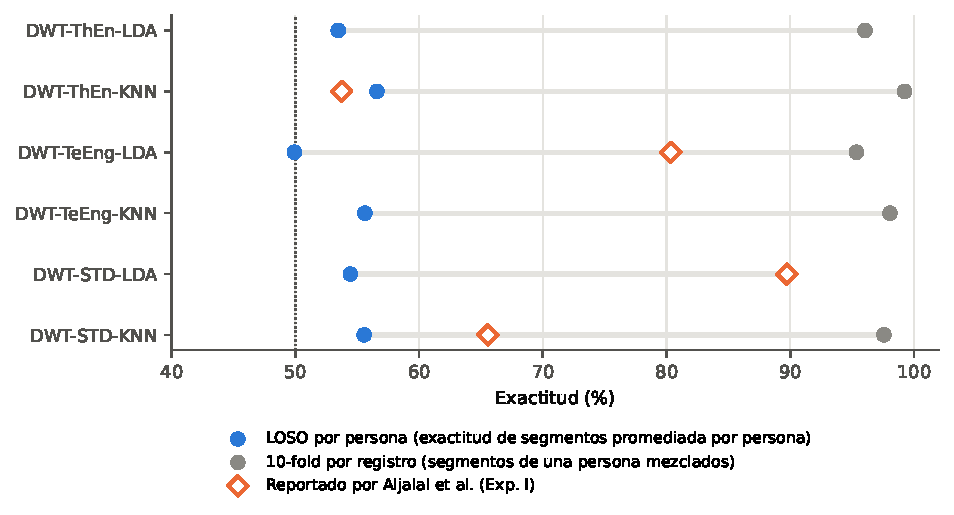
\includegraphics[width=\linewidth]{../figs/es_dev.pdf}
\caption{\textbf{Validación por persona frente a validación por registro en los datos de desarrollo.} Mismas características DWT y clasificadores, 19 canales, EEG\_1 (24 personas). Azul: LOSO, excluyendo del entrenamiento todos los segmentos de la persona evaluada. Gris: validación de 10 particiones sobre segmentos, que mezcla segmentos de la misma persona. Rombos: valores con todos los canales reportados por \citet{aljalal2024} (Experimento I), cuando existen. Línea punteada: 50\,\%.}
\label{fig:dev}
\end{figure}

\paragraph{La selección de electrodos ajusta ruido.} NSGA-II con etiquetas diagnósticas revueltas obtuvo exactitudes LOSO internas de 72--79\,\%, iguales o mayores que con las etiquetas reales (65--75\,\%). En LOSO anidado (DWT-ThEn-KNN), el subconjunto elegido con 23 personas alcanzó 67\,\% internamente, pero 40\,\% en la persona excluida. Con las características más limpias, la regla de selección del artículo obtuvo 48\,\% en LOSO anidado frente a 61\,\% sin selección, y con etiquetas revueltas un método llegó a 71\,\% aun con evaluación anidada, lo que muestra lo amplia que es la distribución del azar con 24 personas.

\paragraph{Los electrodos frontales registran señal ocular.} La fracción de varianza explicada por los componentes oculares de ICA fue de 72\,\% en Fp2, 68\,\% en Fp1, 52\,\% en F7 y 39\,\% en F8, con una caída clara en los demás electrodos. La actividad de movimientos oculares horizontales fue mayor en el grupo MCI ($p=0.015$ sin corregir; exploratorio). Así, dos de los cuatro electrodos que \citet{aljalal2024} eligieron con más frecuencia (Fp1 y F8) están entre los más contaminados.

\paragraph{Las características más limpias no produjeron una señal confiable.} La limpieza con ICA mejoró la exactitud balanceada en unos 9 puntos con todos los tipos de características (de alrededor de 48\,\% a 57\,\%; $p\approx0.14$). En LOSO anidado, M0 obtuvo 61.2\,\% (AUC 0.61) y M4 64.3\,\% (AUC 0.61), ninguno por encima del azar (permutación $p=0.24$ y $0.11$). El AUC \emph{leave-pair-out} de M0 fue 0.65. Con el montaje físico, M0 conservó su exactitud balanceada (61.2\,\%; AUC 0.57; AUC \emph{leave-pair-out} 0.57), pero M4 cayó a 36.7\,\% (AUC 0.29) y eligió una combinación distinta en casi cada pliegue. Estos resultados se conocían antes del preregistro y son la razón por la que H4 no hizo predicción para M4-físico.

\subsection{Prueba externa preregistrada (EEG\_2)}

La prueba se corrió una sola vez, después de enviar el registro, con código y archivos de características cuyas huellas SHA-256 coincidieron con las registradas. La Tabla~\ref{tab:ext} y la Fig.~\ref{fig:main} muestran los resultados.

\begin{table}[t]
\centering\small
\caption{\textbf{Prueba externa preregistrada.} Cada método se ajustó y eligió sus electrodos con EEG\_1 (24 personas) y se evaluó una sola vez con EEG\_2 (34 personas: 18 MCI, 16 controles). Exactitud balanceada con IC bootstrap estratificado del 95\,\%; $p$ de permutación con corrección de Holm sobre los cinco métodos principales. El AUC se da cuando el método produce un puntaje continuo.}
\label{tab:ext}
\begin{tabular}{@{}lccccccc@{}}
\toprule
Método & Electrodos & Aciertos & Sens. (\%) & Espec. (\%) & Exact. balanceada (\%) [IC 95\,\%] & $p_\text{Holm}$ & AUC \\
\midrule
R & 5 & 15/34 & 16.7 & 75.0 & 45.8 [31.2, 60.1] & 1.00 & -- \\
M0 & 15 & 18/34 & 100 & 0 & 50.0 [50.0, 50.0] & 1.00 & 0.52 \\
M4 & 4 & 18/34 & 100 & 0 & 50.0 [50.0, 50.0] & 1.00 & 0.47 \\
M1 & 5\textsuperscript{a} & 18/34 & 100 & 0 & 50.0 [50.0, 50.0] & 1.00 & -- \\
M6 & 5\textsuperscript{a} & 18/34 & 100 & 0 & 50.0 [50.0, 50.0] & 1.00 & -- \\
\midrule
M0-físico & 15 & 18/34 & 72.2 & 31.2 & 51.7 [36.8, 67.0] & --\textsuperscript{b} & 0.44 \\
M4-físico & 4 & 15/34 & 50.0 & 37.5 & 43.8 [28.1, 61.1] & --\textsuperscript{b} & 0.40 \\
\bottomrule
\end{tabular}

\smallskip\footnotesize\raggedright \textsuperscript{a}\,Mediana de cinco semillas (rango 4--5 en M6). \textsuperscript{b}\,No forman parte de la familia de pruebas contra el azar; $p$ de permutación sin corregir $=0.56$ y $0.86$.
\end{table}

\begin{figure}[t]
\centering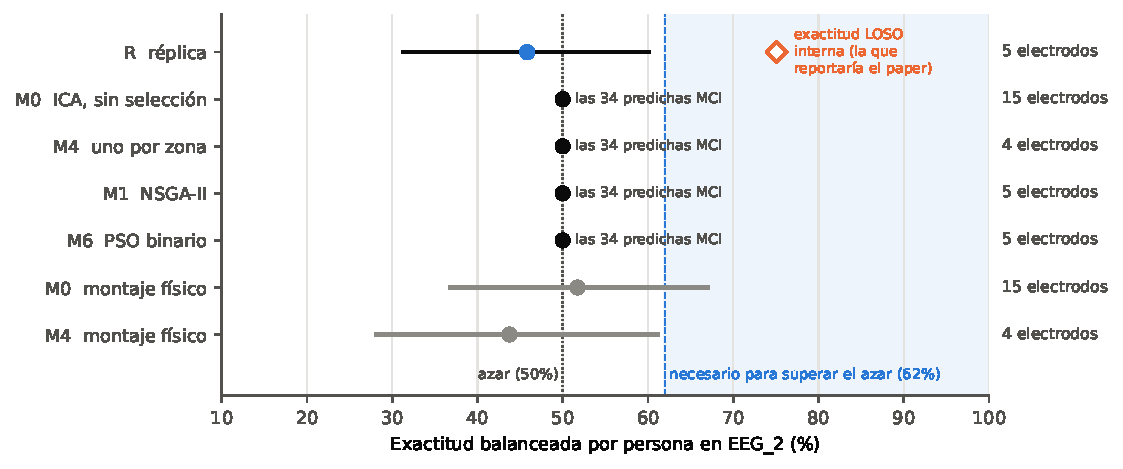
\includegraphics[width=\linewidth]{../figs/es_main.pdf}
\caption{\textbf{Ningún método detectó MCI por encima del azar en personas nuevas.} Exactitud balanceada por persona en EEG\_2 con IC bootstrap del 95\,\%. La zona sombreada es lo que un método necesitaba alcanzar para superar el azar con 34 personas. El rombo es la exactitud LOSO interna de la réplica en EEG\_1, la cifra que reportaría el procedimiento del artículo original. Cuatro métodos predijeron MCI para las 34 personas, por lo que su exactitud es exactamente 50\,\% sin dispersión.}
\label{fig:main}
\end{figure}

\paragraph{PI: ningún método superó el azar.} Tras la corrección de Holm, ningún método superó el azar ($p_\text{Holm}=1.00$ en los cinco). La réplica R clasificó bien a 15 de 34 personas (exactitud balanceada 45.8\,\%), con sensibilidad de 16.7\,\% y especificidad de 75.0\,\%; su exactitud por segmento fue 45.6\,\%. M0, M4, M1 y M6 predijeron MCI para todas las personas de EEG\_2 (sensibilidad 100\,\%, especificidad 0\,\%), un resultado degenerado que se explica en la Sección~\ref{sec:shift}.

\paragraph{H1 se confirmó.} En EEG\_1, NSGA-II eligió T3, Cz, T4, Pz y P4 (dos de ellos, Cz y T4, entre los más elegidos por \citealp{aljalal2024}) con una exactitud LOSO interna de 75.1\,\%, la cifra que reportaría el procedimiento original. Este valor queda por encima del límite superior del IC del 95\,\% de la exactitud balanceada externa (60.1\,\%); la caída fue de 29.3 puntos.

\paragraph{H2 y H3 se cumplieron solo de forma trivial.} M0 resultó formalmente no inferior a R (diferencia $+4.2$ puntos, IC 90\,\% $-7.6$ a $+16.0$, $p=0.026$) y M4 formalmente no inferior a M1 con menos electrodos (4 frente a 5; diferencia 0, $p_\text{Holm}<0.001$). M6 usó la misma mediana de electrodos que M1, así que su parte de H3 no se confirmó. Como M0, M4, M1 y M6 predijeron la misma clase para todas las personas, estas comparaciones no son informativas: muestran que una predicción constante no es peor que R ni que otra predicción constante, no que los métodos más limpios o más parsimoniosos detecten MCI (Fig.~\ref{fig:diff}).

\paragraph{H4 fue no concluyente.} El montaje físico cambió la exactitud balanceada en $+1.7$ puntos para M0 (IC 90\,\% $-10.4$ a $+14.3$; $p_\text{Holm}=0.15$) y en $-6.2$ puntos para M4 ($-20.5$ a $+8.3$; $p_\text{Holm}=0.31$). Ambos intervalos incluyen el margen y el cero, así que no se demostró la no inferioridad ni tampoco la inferioridad.

\begin{figure}[t]
\centering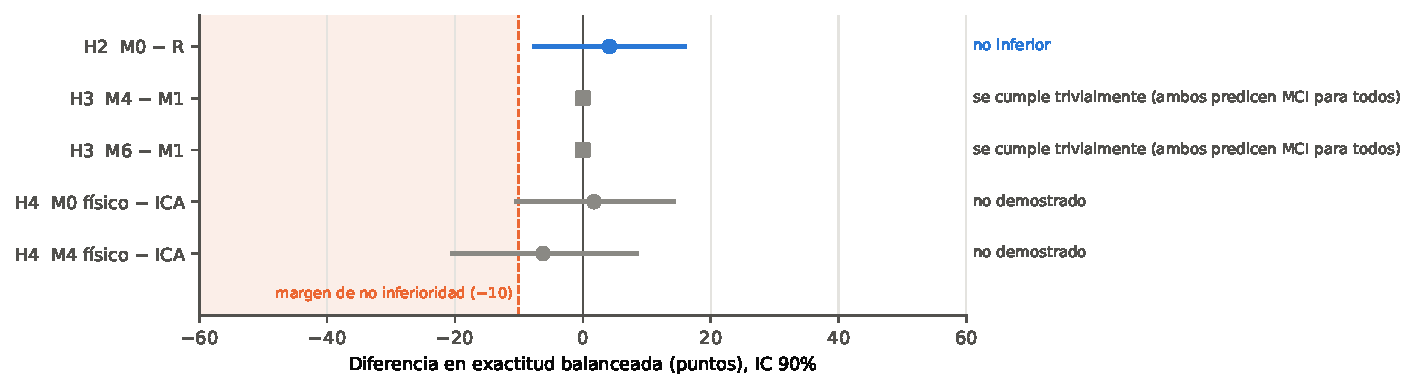
\includegraphics[width=\linewidth]{../figs/es_diff.pdf}
\caption{\textbf{Comparaciones pareadas preregistradas.} Diferencia en exactitud balanceada en las mismas 34 personas con IC bootstrap pareado del 90\,\%; la no inferioridad requería que el límite inferior quedara por encima de $-10$ (línea discontinua). Los cuadrados marcan comparaciones entre dos métodos que predijeron MCI para todos, que se cumplen de forma trivial.}
\label{fig:diff}
\end{figure}

\subsection{Por qué fallaron los métodos: cambio de dominio y confusores de adquisición}\label{sec:shift}

\paragraph{Las dos bases se distinguen casi perfectamente.} El control descriptivo identificó la base de origen de las 58 personas a partir de sus características de 15 electrodos con 94.4\,\% de exactitud balanceada, muy por encima del umbral de 75\,\% que registramos para un cambio de dominio grande. En EEG\_2 la banda delta concentró en promedio el 68.8\,\% de la potencia de 1--30\,Hz, frente a 39.7\,\% en EEG\_1, mientras que alfa bajó de 21.7\,\% a 8.0\,\% (Fig.~\ref{fig:conf}, izquierda). En EEG\_1 el grupo MCI tenía más delta que los controles (43.5\,\% frente a 36.4\,\%), así que todos los modelos aprendieron que más delta significa MCI; al aplicarlos a EEG\_2, donde todos tienen más delta que cualquier persona de EEG\_1, asignaron a las 34 personas a MCI. Dentro de EEG\_2 la dirección se invirtió (67.1\,\% en MCI frente a 70.7\,\% en controles).

\begin{figure}[t]
\centering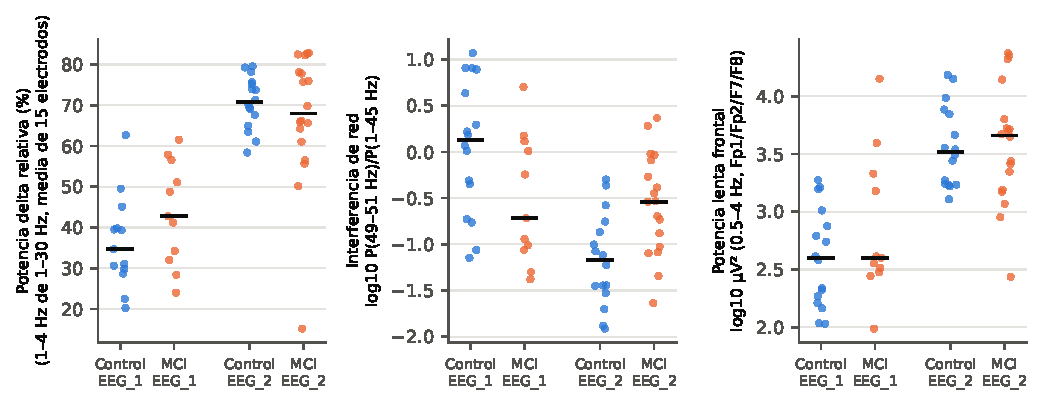
\includegraphics[width=\linewidth]{../figs/es_conf.pdf}
\caption{\textbf{Las diferencias entre bases son mayores que las diferencias entre grupos.} Cada punto es una persona; las barras son medianas. Izquierda: potencia delta relativa, la característica que mueve a los clasificadores. Centro: interferencia de la red eléctrica en los registros originales; su asociación con el diagnóstico se invierte entre bases. Derecha: potencia lenta frontal, unas nueve veces mayor en EEG\_2.}
\label{fig:conf}
\end{figure}

\paragraph{La interferencia de la red se asocia con la etiqueta, en sentidos opuestos.} La potencia relativa en 49--51\,Hz de los registros originales difirió entre bases ($p<0.001$) y se asoció con el diagnóstico en ambas, pero en sentidos opuestos: en EEG\_1 los controles tenían más interferencia que los MCI (AUC 0.28 de la interferencia como predictor de MCI; $p=0.064$), mientras que en EEG\_2 los MCI tenían más interferencia que los controles (AUC 0.79; $p=0.004$). Las condiciones de adquisición están entrelazadas con los grupos diagnósticos de una forma que no se transfiere entre bases.

\paragraph{Los puntajes de los modelos siguen a la actividad lenta frontal.} La potencia lenta frontal (0.5--4\,Hz en Fp1, Fp2, F7 y F8) fue unas nueve veces mayor en EEG\_2 ($p<0.001$) y no difirió entre grupos dentro de ninguna base. En EEG\_2, el puntaje continuo de M0 se correlacionó con esta potencia lenta frontal (Spearman $\rho=0.42$, $p=0.012$) y no significativamente con el diagnóstico (AUC 0.52), aun cuando los electrodos frontales se habían eliminado y los componentes oculares restado.

\subsection{Análisis exploratorios}

\paragraph{Tampoco hay señal de ordenamiento.} El AUC, que no depende del umbral de decisión y por tanto no se ve afectado por un desplazamiento global, fue 0.52 para M0, 0.47 para M4, 0.44 para M0-físico y 0.40 para M4-físico. Entrenar con las 27 personas de EEG\_1 no cambió el panorama (AUC 0.41--0.54). En un análisis \emph{post hoc} no preregistrado, estandarizar cada base con su propia media y desviación estándar (sin etiquetas) eliminó el desplazamiento global pero no reveló señal: AUC 0.52 para M0 ($p=0.44$) y 0.45 para M4 con ICA, 0.42 y 0.38 con el montaje físico.

\paragraph{El control positivo apuntó en la dirección esperada, pero fue débil.} La potencia alfa relativa posterior fue menor en MCI que en controles en ambas bases, como se esperaba \citep{babiloni2015}, pero el efecto fue pequeño y no significativo (AUC 0.59, $p=0.49$ en EEG\_1; 0.57, $p=0.48$ en EEG\_2; similar con el montaje físico).

\paragraph{Los electrodos elegidos fueron estables pero no válidos.} M1 eligió el mismo subconjunto (F4, T4, T5, Pz, T6) con cuatro de cinco semillas, y M6 eligió T4 y T6 con las cinco semillas y F4 y Pz con cuatro (Fig.~\ref{fig:heads}). Esta estabilidad entre semillas no se tradujo en desempeño externo.

\begin{figure}[t]
\centering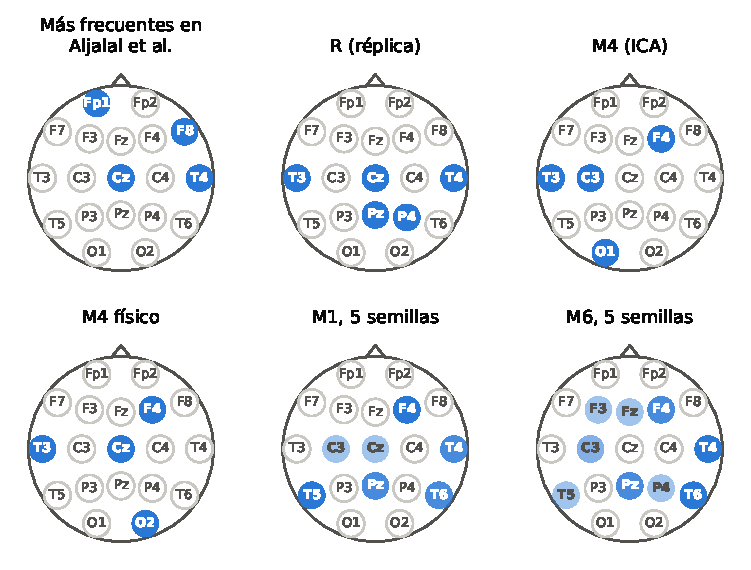
\includegraphics[width=0.82\linewidth]{../figs/es_heads.pdf}
\caption{\textbf{Electrodos elegidos en EEG\_1.} Más oscuro significa elegido con más frecuencia (entre semillas en M1 y M6). Fp1 y F8, dos de los electrodos más elegidos por \citet{aljalal2024}, están entre los más contaminados por movimientos oculares; M0--M6 excluyen Fp1, Fp2, F7 y F8 por diseño.}
\label{fig:heads}
\end{figure}

\section{Discusión}

En una prueba externa preregistrada, una réplica independiente de la selección de electrodos con NSGA-II para detectar MCI alcanzó 75.1\,\% de exactitud interna con cinco electrodos y 45.8\,\% de exactitud balanceada en 34 personas que nunca había visto. Cuatro alternativas construidas para evitar los problemas conocidos no lo hicieron mejor: todas clasificaron a cada persona nueva como MCI. Ningún método, con ningún número de electrodos ni con ninguno de los dos montajes, detectó MCI por encima del azar en la cohorte nueva.

\paragraph{De dónde vienen las exactitudes publicadas.} Tres mecanismos, cada uno medido en los datos de desarrollo, pueden explicar la diferencia entre las exactitudes publicadas y nuestros resultados. Primero, cuando segmentos de la misma persona se usan para entrenar y probar, se alcanzan exactitudes de 90--99\,\% con características que dan resultados al nivel del azar cuando las personas se mantienen separadas; la cifra con todos los canales reportada por \citet{aljalal2024} está más cerca de lo primero. Con el artículo no podemos saber cómo se construyeron los pliegues, así que esta es una afirmación de compatibilidad, no sobre su código. Segundo, NSGA-II alcanza 72--79\,\% de exactitud interna con etiquetas revueltas, así que una exactitud interna de 75\,\% después de la selección no aporta evidencia de valor diagnóstico; la evaluación anidada y la prueba externa eliminan este sesgo \citep{varma2006,cawley2010}. Tercero, dos de los electrodos elegidos con más frecuencia (Fp1 y F8) están dominados por señal ocular. Estos mecanismos no requieren ningún error en el análisis original: son el comportamiento esperado de una búsqueda sin restricciones evaluada en las mismas 24 personas, y por eso los atendimos por diseño y probando en personas nuevas.

\paragraph{El cambio de dominio domina.} El hallazgo más informativo no estaba planteado como hipótesis: dos bases públicas del mismo centro y sistema de registro se distinguen en 94\,\% solo por su EEG, y la diferencia (un espectro dominado por delta en EEG\_2, nueve veces más potencia lenta frontal y un perfil distinto de interferencia de red) es mayor que cualquier diferencia entre MCI y controles. Con los archivos publicados no podemos determinar su causa; la vigilancia, la impedancia de los electrodos, el filtrado o el periodo de registro son explicaciones posibles. Su consecuencia, en cambio, es clara: un modelo que aprendió una pequeña diferencia de potencia delta entre grupos moverá a toda la cohorte nueva al otro lado de su frontera de decisión. La estandarización por base eliminó el desplazamiento global pero no reveló señal residual, así que el fallo no es solo un problema de calibración. La asociación opuesta entre la interferencia de red y el diagnóstico en las dos bases muestra que las condiciones de adquisición pueden confundirse con los grupos. En bases tan pequeñas, cualquier método que busque ampliamente, ya sea que optimice electrodos, características o clasificadores, probablemente encontrará estos confusores.

\paragraph{Qué lograron y qué no las alternativas más limpias.} Las alternativas se diseñaron para eliminar tres fuentes de optimismo: la fuga entre segmentos, el sesgo de selección y la contaminación ocular. Lo lograron en el sentido de que sus estimaciones internas fueron honestas (alrededor de 61--64\,\% en LOSO anidado, nunca por encima del azar), pero no crearon una señal que no existe en estos datos. Las confirmaciones formales de H2 y H3 no son evidencia de que funcionen; solo muestran que su fallo no fue peor que el del método original. La selección parsimoniosa al menos no perjudicó, y los electrodos que eligieron NSGA-II y PSO fueron estables entre semillas. Sin embargo, la estabilidad no implicó validez: un subconjunto estable puede estar ajustado de forma estable a un confusor.

\paragraph{Electrodos virtuales frente a físicos.} Los estudios de minimización de electrodos suelen calcular cada canal después de una referencia promedio y una ICA sobre el montaje completo, y luego reportan los canales elegidos como si un dispositivo pudiera usarlos solos. El montaje físico pone esto a prueba directamente. En desarrollo, el método de un electrodo por zona perdió la mayor parte de su exactitud con electrodos físicos; en la prueba externa la comparación fue no concluyente porque ninguno de los dos montajes funcionó. Recomendamos que los estudios futuros reporten ambas versiones.

\paragraph{Recomendaciones.} A partir de estos resultados proponemos el siguiente protocolo mínimo para estudios que eligen electrodos de EEG con fines diagnósticos: evaluar por persona, nunca por segmento; mantener la selección dentro del ciclo de validación (anidada); comparar contra el mismo procedimiento corrido con etiquetas revueltas; reportar el AUC además de la exactitud; revisar si los electrodos elegidos están contaminados por movimientos oculares y si variables de adquisición (como la interferencia de red) difieren entre grupos; reportar una versión con montaje físico; probar si las bases se pueden distinguir antes de combinarlas o transferir modelos entre ellas; y preregistrar una prueba externa única \citep{nosek2018,collins2024}.

\paragraph{Limitaciones.} Los tamaños de muestra son pequeños, así que la prueba externa solo podía detectar efectos grandes (potencia de 0.84 para una exactitud balanceada real de 70\,\%) y las hipótesis no confirmadas son no concluyentes más que negativas. EEG\_2 se publicó como extensión de la misma base, pero no pudimos verificar que sus criterios diagnósticos y de inclusión, su protocolo de registro o su periodo sean idénticos, y la causa del cambio de dominio sigue sin conocerse. Nuestra réplica descansa en supuestos documentados donde el artículo original no es específico (familia wavelet, umbral de entropía, operadores genéticos, qué controles se excluyeron), y la prueba externa cubrió la mejor configuración de selección de canales del artículo (DWT, ThEn, análisis discriminante), no todas las combinaciones de características ni la selección conjunta de características de su Experimento III. Solo se analizaron los primeros 10 minutos de cada registro, no había información de edad ni sexo y la regla de componentes de ICA fue automática. Algunos diagnósticos de desarrollo (etiquetas revueltas, contaminación ocular) se calcularon antes del registro y se reportan como resultados de desarrollo. Por último, la estandarización por base fue \emph{post hoc}. Ninguna de estas limitaciones favorece la conclusión de que las exactitudes originales se transfieren: si acaso, cada una facilitaría encontrar una señal transferible.

\section{Conclusiones}

Las altas exactitudes reportadas para la selección de electrodos con NSGA-II en la detección de MCI con EEG en reposo no sobrevivieron a una prueba externa independiente y preregistrada: una exactitud interna de 75\,\% se convirtió en 46\,\% en personas nuevas, y ninguna de cuatro alternativas más limpias o más parsimoniosas superó el azar. El factor decisivo fue un gran cambio de dominio entre dos bases del mismo centro, junto con variables de adquisición asociadas a los grupos diagnósticos. Minimizar electrodos solo tiene sentido una vez que se demostró que una señal generaliza; hasta entonces, recomendamos una evaluación por persona, anidada y validada externamente, con montajes físicos y análisis preregistrados.


\section*{Preregistro}
Las hipótesis, las reglas de decisión, el código y las huellas de las características de prueba se registraron en OSF antes de la prueba externa: \url{https://osf.io/4enh8}. Desviaciones: ninguna en el análisis confirmatorio. La estandarización por base de los análisis exploratorios se agregó después de ver los resultados y se marca como \emph{post hoc}.

\section*{Disponibilidad de datos}
Ambas bases están disponibles públicamente en la Universidad de Ciencias Médicas de Isfahan, en \url{https://misp.mui.ac.ir/en/eeg-data} \citep{kashefpoor2016,kashefpoor2019}. Los archivos de características extraídas pueden regenerarse bit a bit con el código publicado; sus huellas SHA-256 están en el preregistro.

\section*{Disponibilidad del código}
El código completo (réplica, métodos congelados, montaje físico, reglas de decisión, análisis exploratorios y figuras) está disponible en el registro de OSF y en el repositorio público que acompaña al artículo.

\section*{Declaración ética}
Este es un análisis secundario de datos públicos y anonimizados. Los estudios originales obtuvieron aprobación ética y consentimiento informado según se reporta en sus publicaciones \citep{kashefpoor2016,kashefpoor2019}.

\section*{Contribuciones de las autoras y el autor}
\textbf{J.M.C.R.}: conceptualización, metodología, software, investigación, análisis formal, redacción del borrador original. \textbf{A.C.T.V.}: conceptualización, metodología, software, validación, análisis formal, visualización, redacción del borrador original, revisión y edición. \textbf{S.M.H.C.}: supervisión, revisión y edición. Todas las personas autoras aprobaron el manuscrito final.

\section*{Financiamiento}
Esta investigación no recibió financiamiento específico.

\section*{Conflicto de intereses}
Las personas autoras declaran no tener conflictos de intereses.

\bibliographystyle{unsrtnat}
\bibliography{../shared/refs}

\end{document}
